\documentclass[12pt]{article}
\usepackage{amsmath,amssymb,amsthm}
\usepackage[english]{babel}
\usepackage[utf8]{inputenc}
\usepackage{fancyhdr}
\usepackage{changepage} 

% for line spacing
\usepackage{setspace}

% for absolute value
\usepackage{commath}

% for numbering
\usepackage{enumerate}

% for image placing
\usepackage{float}

% paper size and margins
\usepackage[letterpaper, left=20mm, right=20mm, top=25mm, bottom = 25mm, headsep=.15in]{geometry}

% for code snippet
\usepackage{listings}

% for curly brace
\usepackage{amsmath}

% for input images
\usepackage{graphicx}
\graphicspath{ {./} }
\usepackage{subfig}

% for printing pseudocode
\usepackage[boxed]{algorithm}
\usepackage[noend]{algpseudocode}

% for tables
\usepackage{tabularx}

\makeatletter
\def\BState{\State\hskip-\ALG@thistlm}
\makeatother

% for circled numbers
\usepackage{tikz}
\newcommand*\circled[1]{\tikz[baseline=(char.base)]{
            \node[shape=circle,draw,inner sep=1pt] (char) {#1};}}

% double line space
\renewcommand{\baselinestretch}{2.0}

% header, footer and page number
\pagestyle{fancy}
\fancyhf{}
\rhead{Tiankai Jiang \quad 20834939}
\lhead{ECE657A \quad Assignment 2}
\fancyfoot[C]{\thepage}

\setlength{\headheight}{15pt}
\lstset{language=Python}
\begin{document}
\noindent
\textbf{\large Question 3:}\\
\begin{center}
    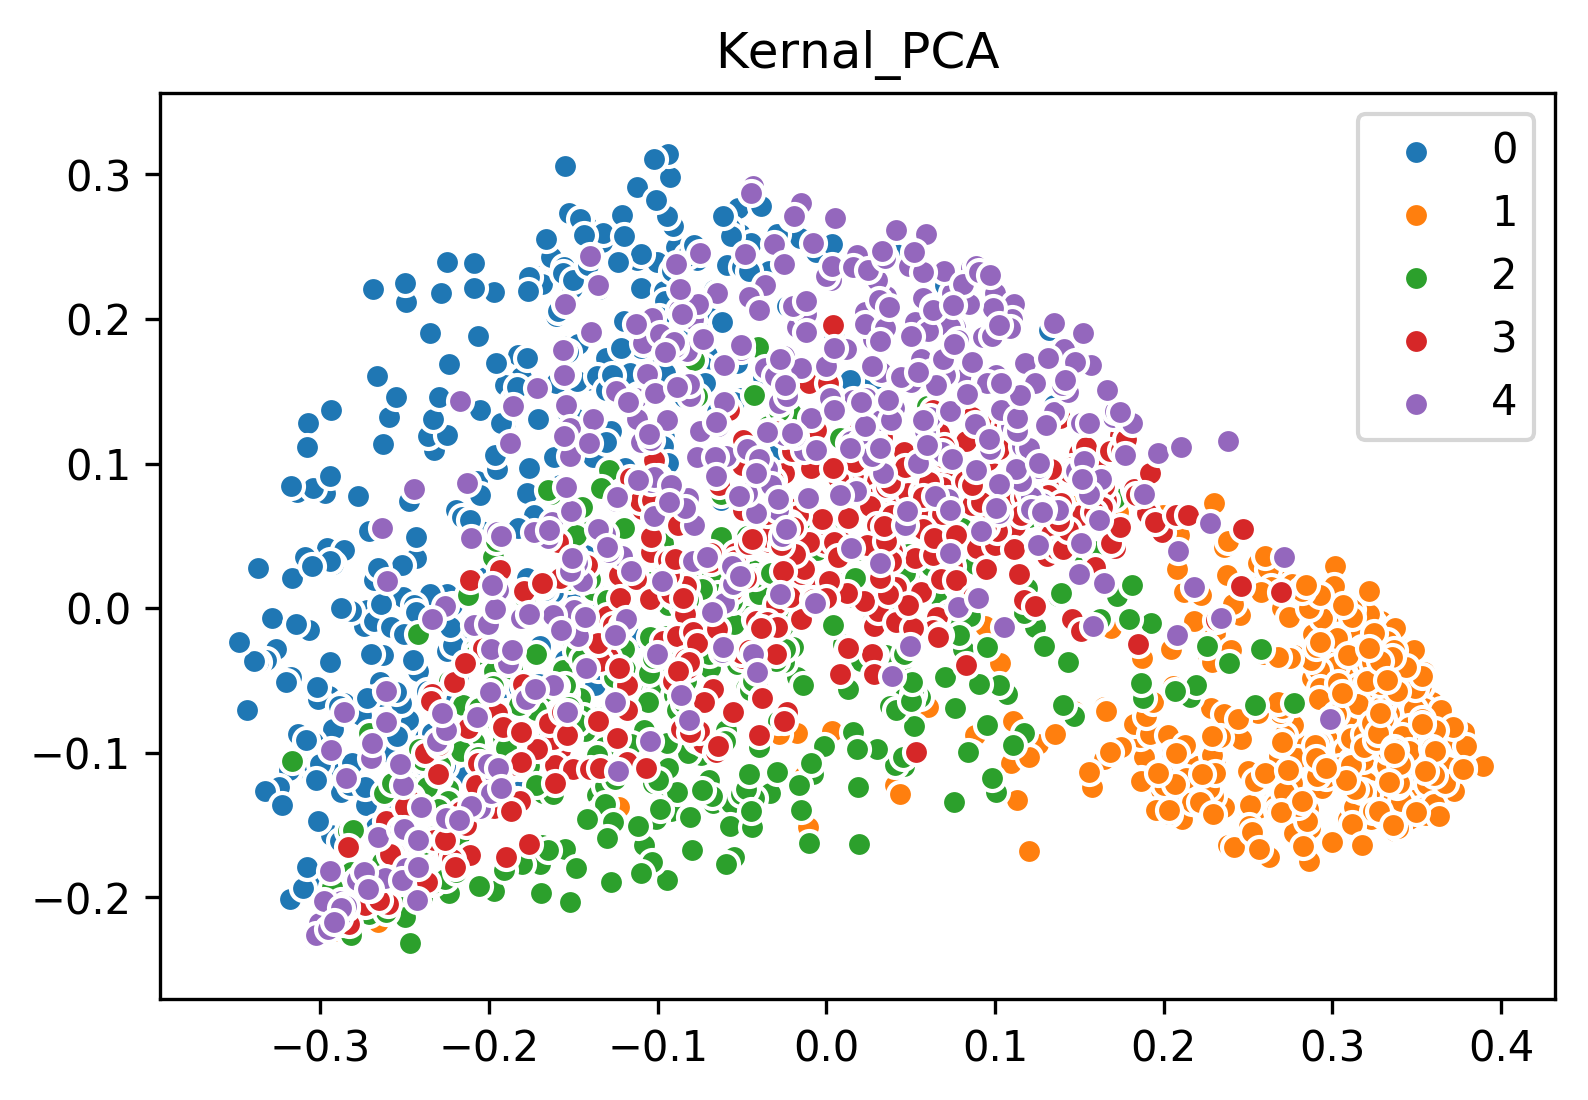
\includegraphics[width=15cm]{Q3_Kernal_PCA.png}
    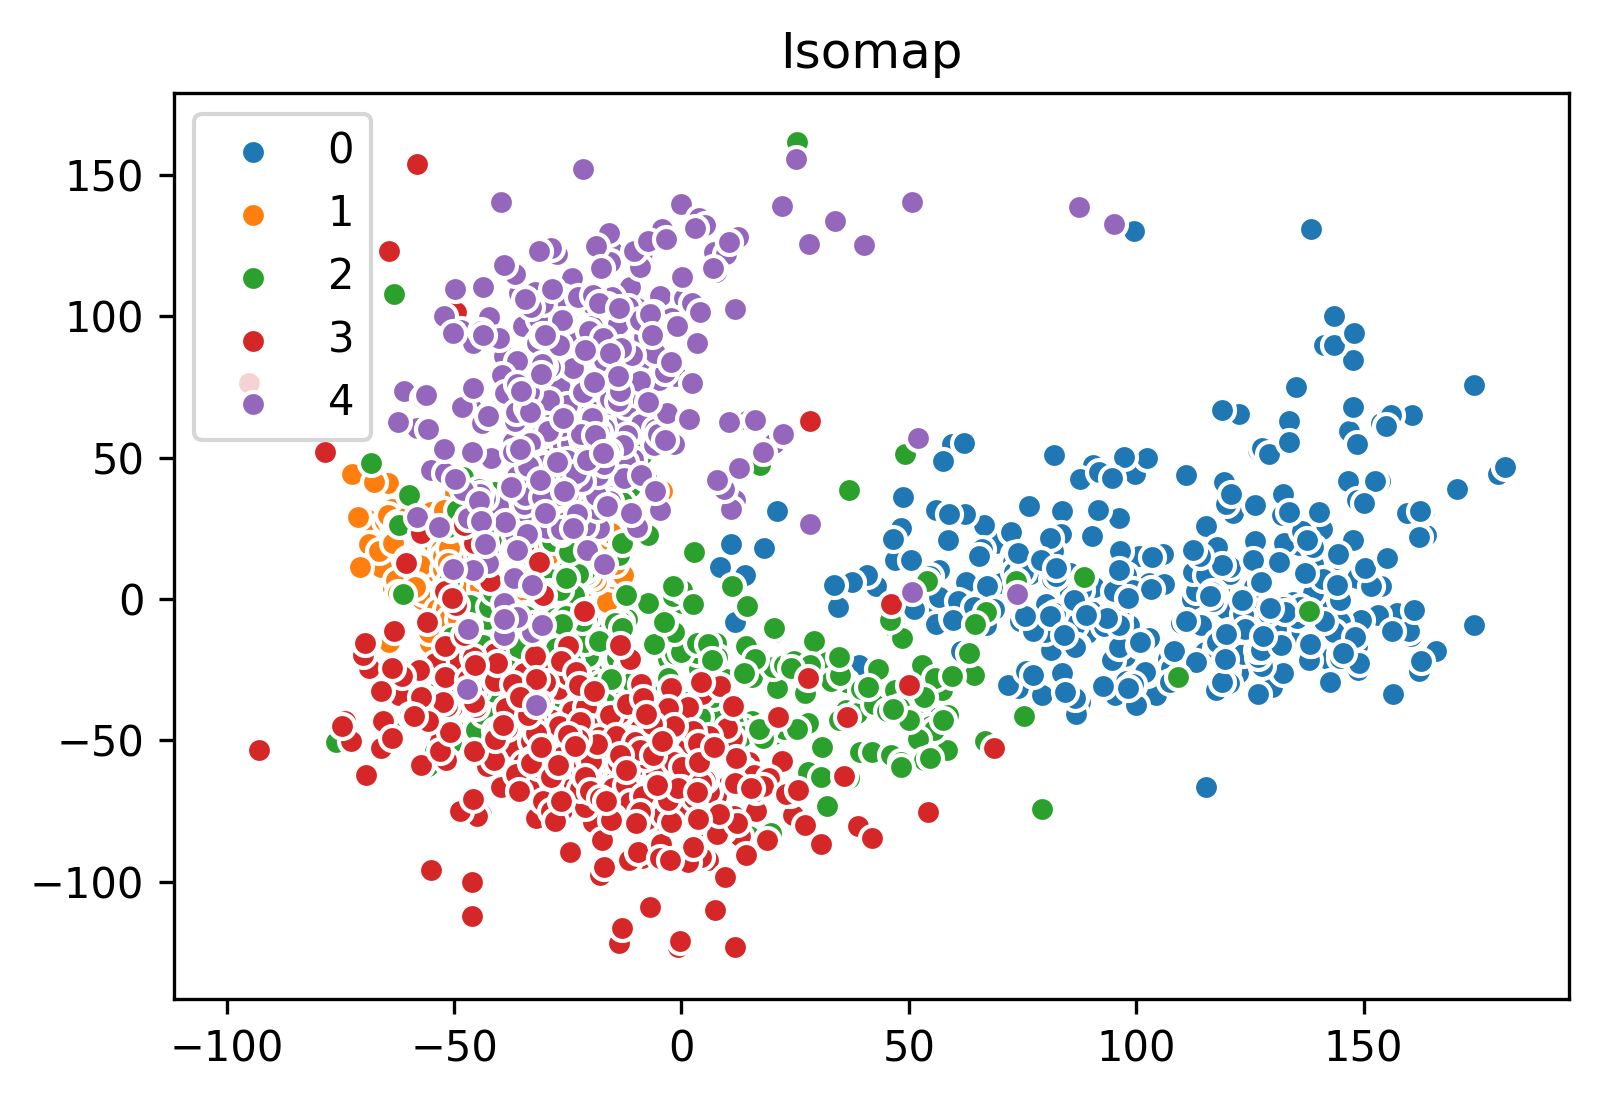
\includegraphics[width=15cm]{Q3_Isomap.png}
    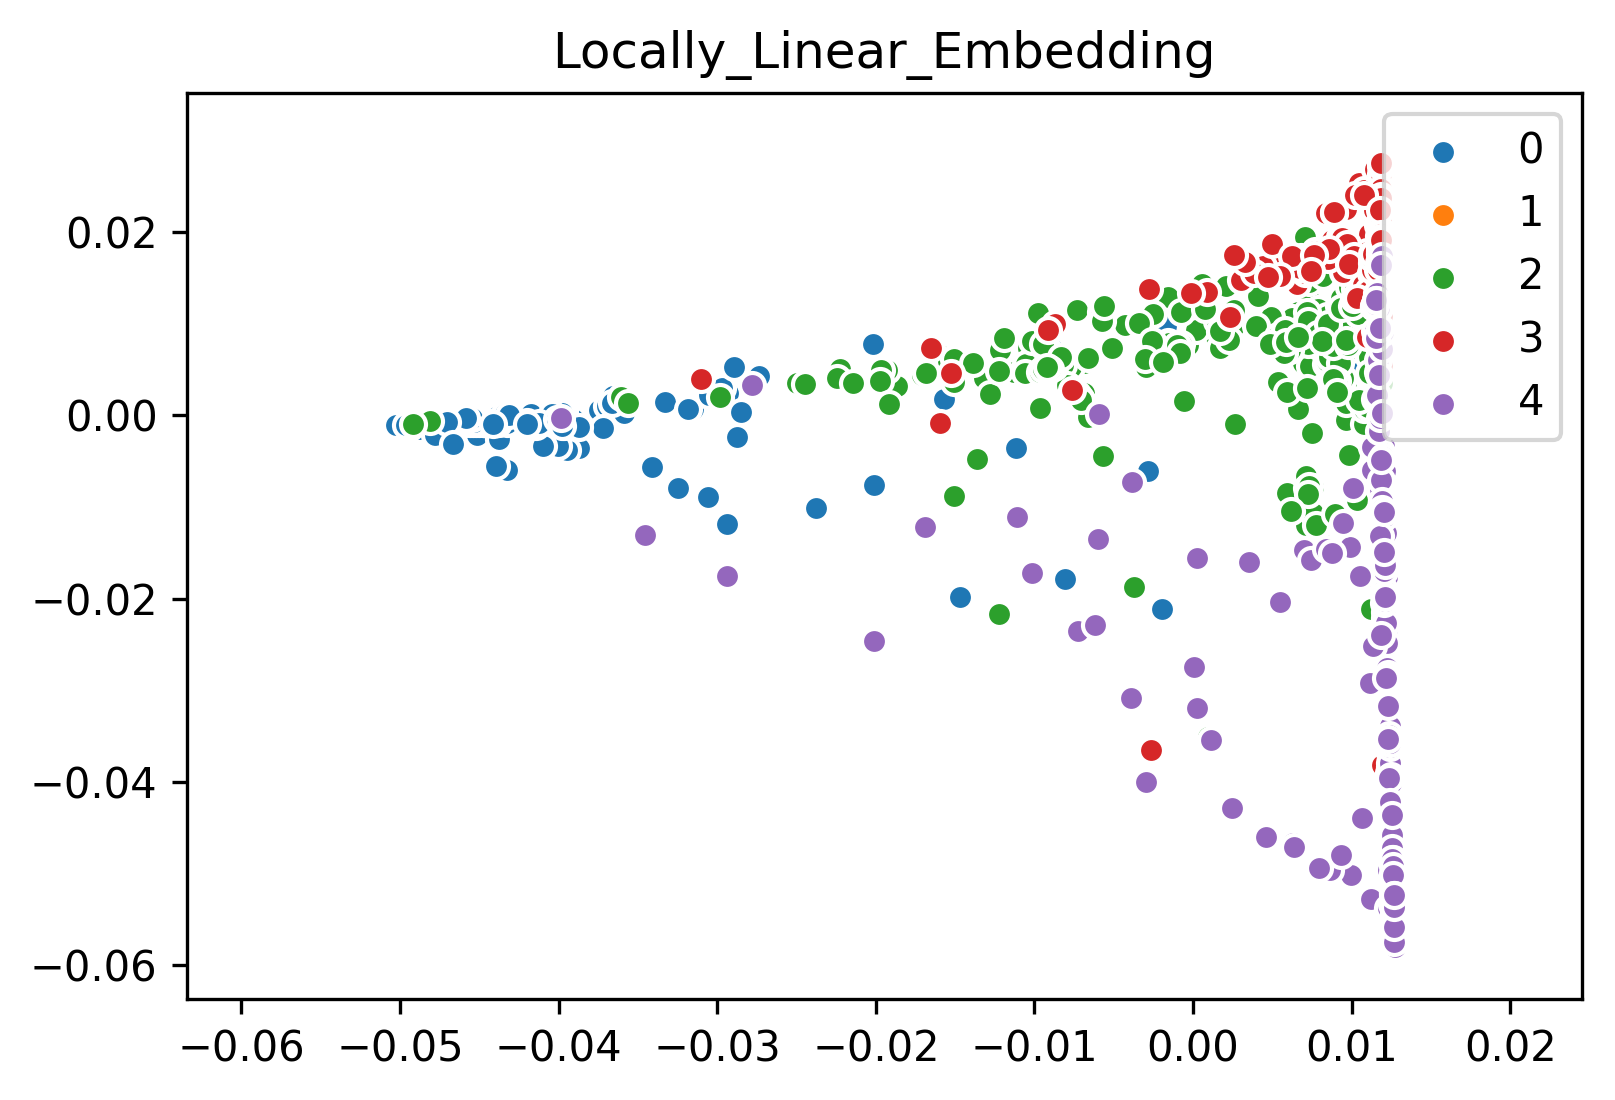
\includegraphics[width=15cm]{Q3_Locally_Linear_Embedding.png}
    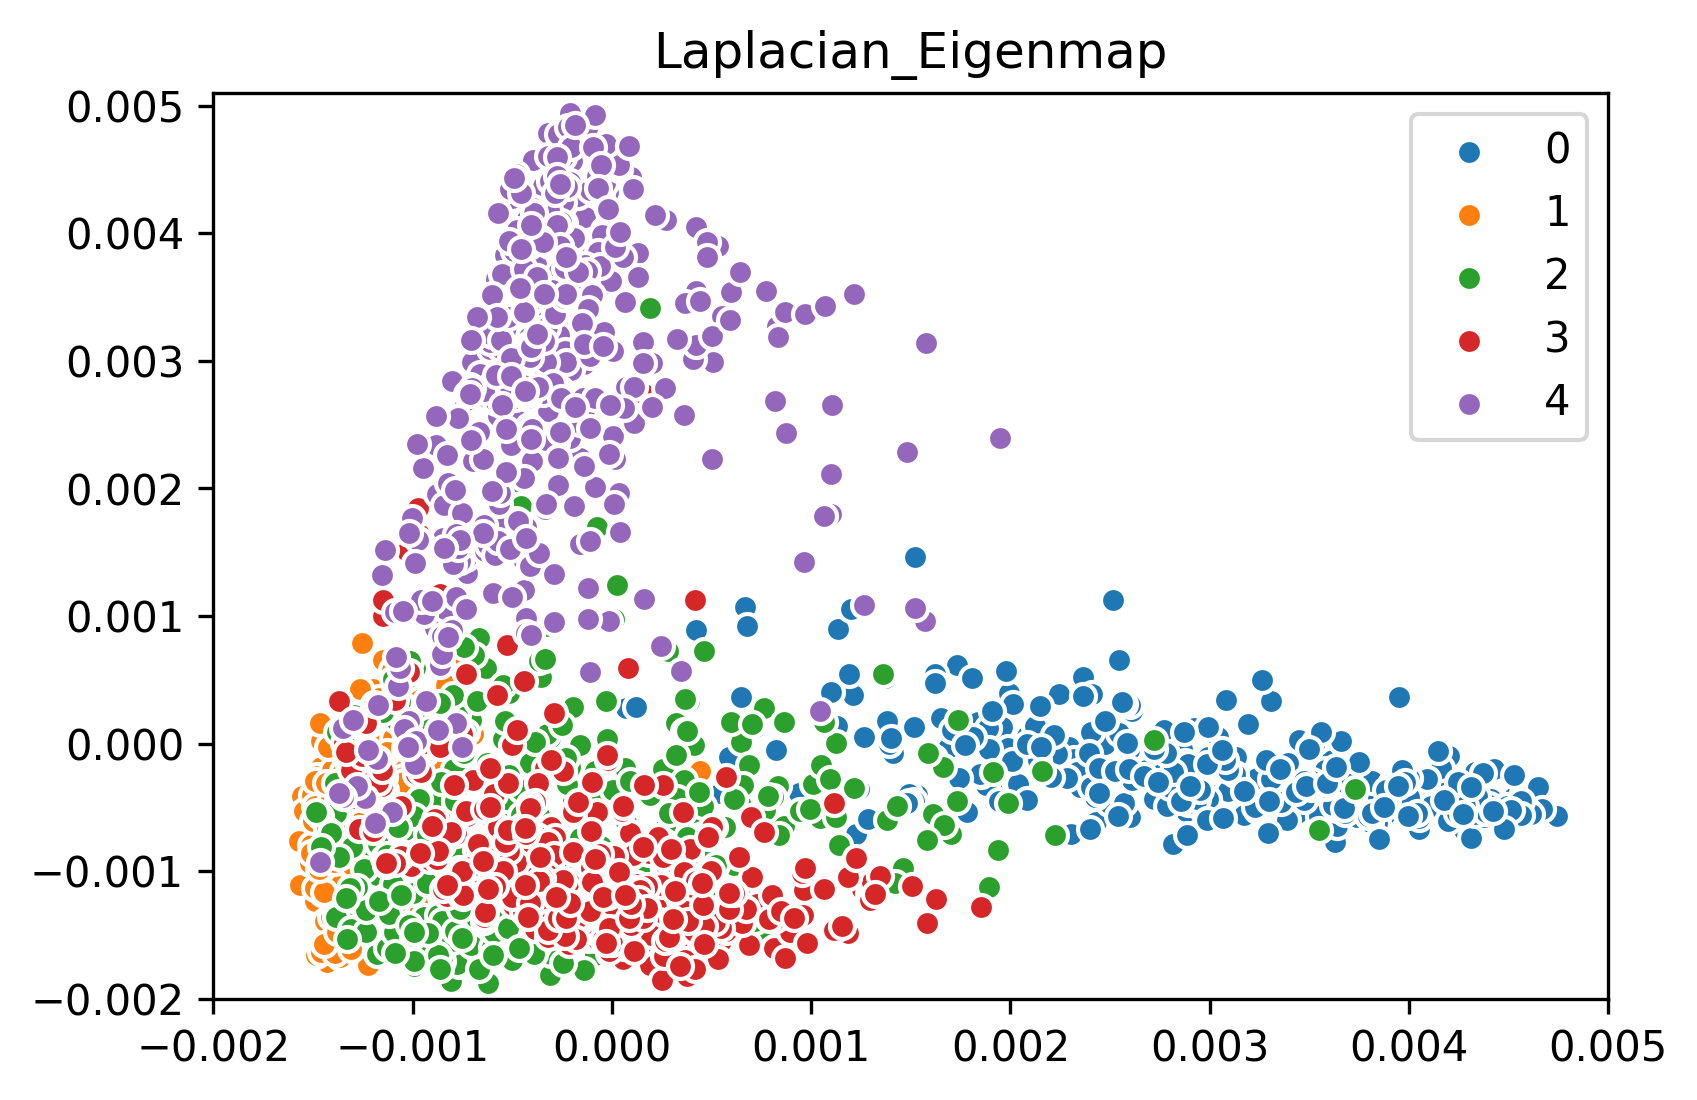
\includegraphics[width=15cm]{Q3_Laplacian_Eigenmap.png}
    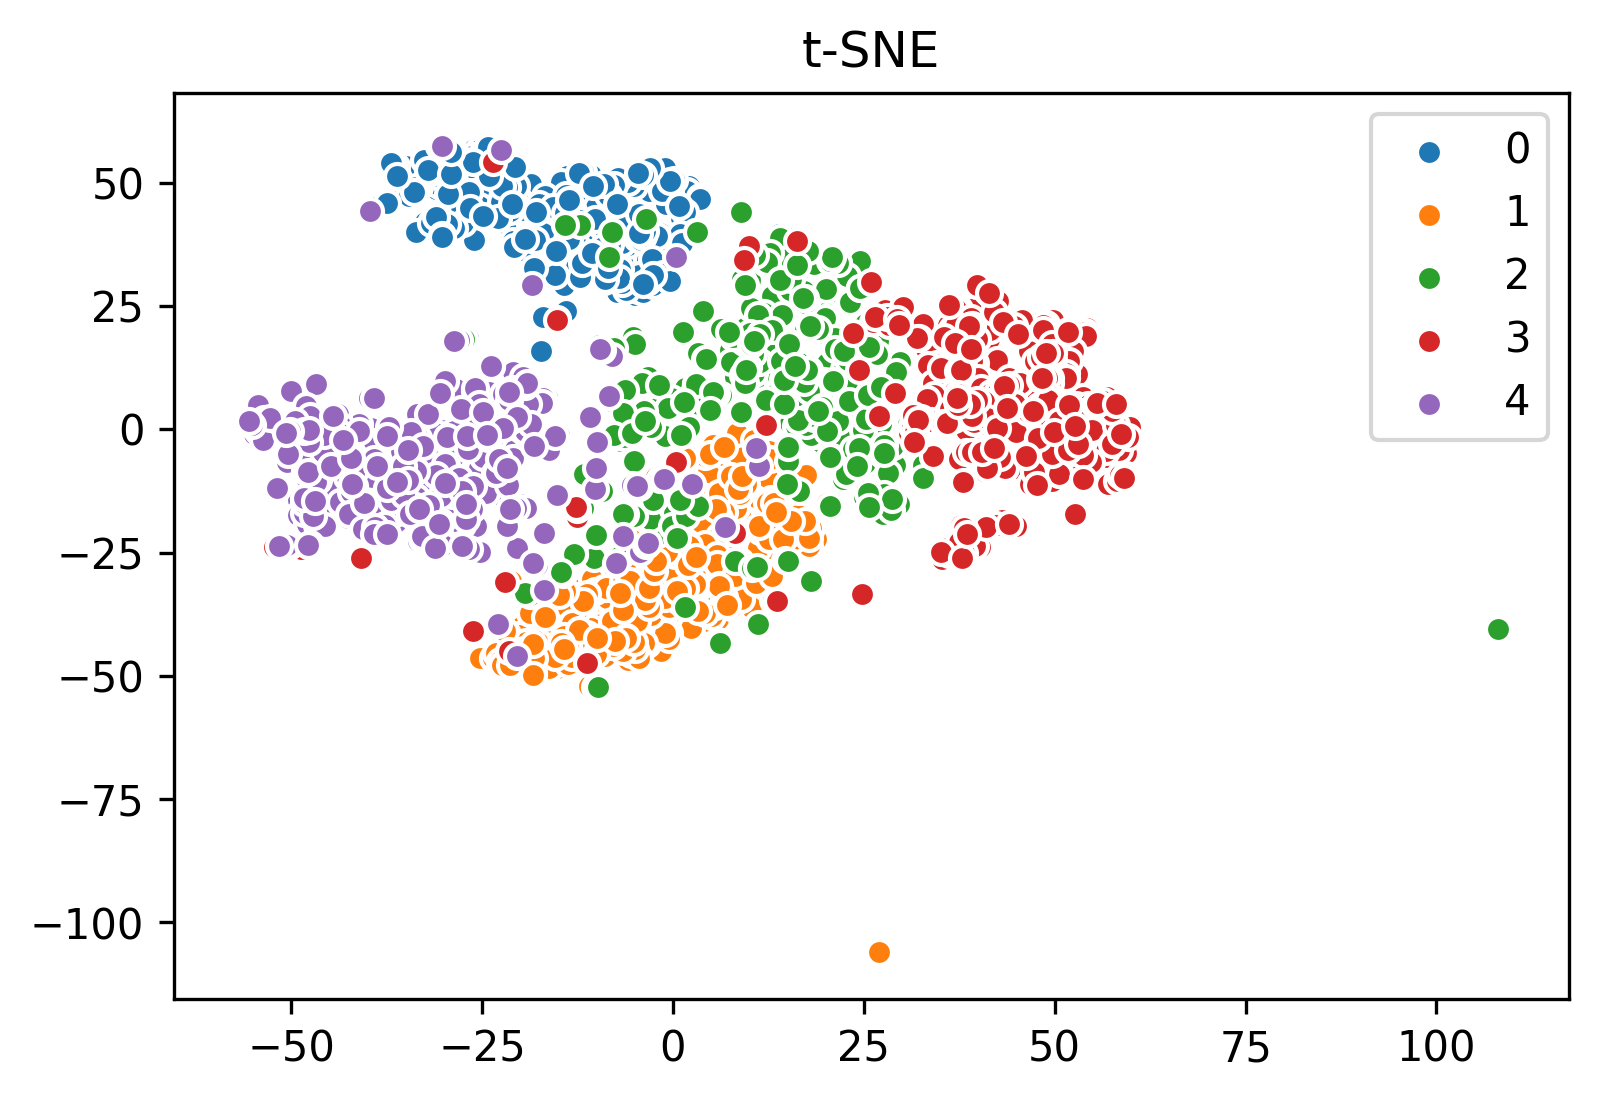
\includegraphics[width=15cm]{Q3_t-SNE.png}
\end{center}
\noindent
\textbf{Which methods do better on which parts of the data?}\\
Kernal PCA does better on number 1. Isomap, LLE and Laplacian Eigenmap does better on number 0 and number 4. t-SNE does better on all classes.\\\\
\textbf{Give at least three clear performance differences between a pair of methods that you can explain based on the nature of methods and the data.}\\
t-SNE is more than 30 times slower than kernal PCA since t-SNE places the points randomly at the beginning and move each point a little bit based on its similarity with other points and the whole process contains hundreds/thousands of iteration so overall it is relatively show.\\\\
Each class of points in Isomap distributes adjacently on the plot and there is little overlap between each two classes. E.g. points of number 1 is below number 4, points of number 3 is below number 1 and points of number 2 are on number 0's left... Unlike kernel PCA, in which multiple classes overlap in the same area. This is because Isomap preserves locality. If two classes have some similar characters in a higher dimension and they lies next to each other, that relation will be preserved in the lower dimension and be reflected on the plot.\\\\
In the plot of Local Linear Embedding, most of the points distribute on the border of a triangle, while the distribution of points of kernel PCA is relatively uniform. This is because the solution of kernel PCA is $\Sigma V^T$, which is the product of diagonal eigenvalues and the eigenvectors. However, the solution of LLE is the second to the (p+1)th smallest eigen values of $(I-W)(I-W)^T$, which is not stretched in space by eigenvalues. Therefore, points are more likely to concentrate on a line and form a hollow on the plot.\\\\
\textbf{What tradeoffs might need to be considered in order to decide which method is ’best’ to use for this dataset?}\\
Efficiency: t-SNE has the best solution quality, but it takes 30 times longer to solve the problem comaparing to kernel PCA. And other 3 methods takes 10 times longer than kernel PCA. If the dataset is large, using t-SNE will not be a good idea though it classifies data well.\\\\
Hyperparameters: for t-SNE, a proper learning rate and iteration should be chosen and for LLE and Isomap, a proper n-neighbor should be chosen. An algorithm cannot be considered as the best method if its hyperparameters are too difficult to tune.\\\\
Encoding: For kernel PCA, we can encode out of sample points using $y=\Sigma^{-1}V^TK(X,x)$. But for LLE, Isomap and Laplacian Eigenmap, we cannot encode them since their kernel is expressed by a piece of code instead of a closed form.\\\\
Sample size: for algorithms that preserves locality such as Isomap, if the samples are sparse in space, there will be discontinuity when the algorithm tries to unfold data to a lower dimension and the algorithm will not perform well.
\end{document}